%%%%%%%%%%%%%%%%%%%%% chapter.tex %%%%%%%%%%%%%%%%%%%%%%%%%%%%%%%%%
%
% sample chapter
%
% Use this file as a template for your own input.
%
%%%%%%%%%%%%%%%%%%%%%%%% Springer-Verlag %%%%%%%%%%%%%%%%%%%%%%%%%%
%\motto{Use the template \emph{chapter.tex} to style the various elements of your chapter content.}
\chapter{其他生物特征识别}
\label{basic} % Always give a unique label
% use \chaptermark{}
% to alter or adjust the chapter heading in the running head

随着移动互联网、智能移动终端设备的快速发展,由于具备便捷的使用体验、可靠的安全保障,以人脸识别为代表的生物特征识别技术(biometrics)得到了迅速应用和推广。生物特征识别技术是利用固有的生物特征进行身份认证的一类技术,由于生物特征通常具备唯一性,如果具备可测量和可验证,那么利用生物识别技术进行身份认证往往安全、可靠和准确。除了前面介绍的人脸识别之外,下面将介绍几种在金融行业应用的生物识别技术以及应用场景。



\section{指纹/掌纹识别}

作为生物识别技术在金融领域应用最早的一项技术,指纹识别早在上世纪90年代就大规模进军金融行业。指纹是人类手指末端由凹凸的皮肤所形成的纹路,如图\ref{fig:fingerprint_img}所示,每个个体指纹的形状不会随着年龄发生改变,而且每个人的指纹都是不同的。指纹识别技术通过分析所采集的指纹图像中可测量的特征点并提取特征值,然后进行比对认证。指纹识别目前也早已在消费电子、安防等领域广泛应用,相关针对指纹的国家标准也已陆续制定和发布,指纹识别的性能已得到明显提高,技术也最为成熟,目前已处于应用成熟的平台期。

\begin{figure}[ht]
\centering  %图片全局居中
\subfigure[指纹采集设备]{
\label{fig:fingerprint_equip}
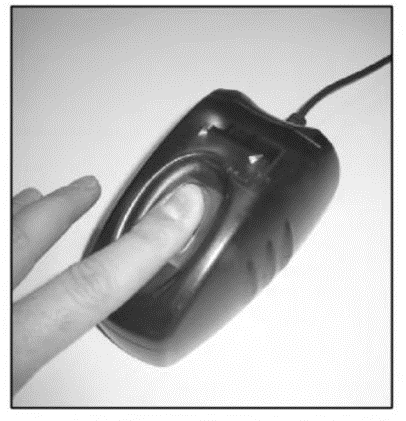
\includegraphics[height=0.45\textwidth]{img/chapter_br/fingerprint_equip.png}}
\subfigure[指纹图像]{
\label{fig:fingerprint_img}
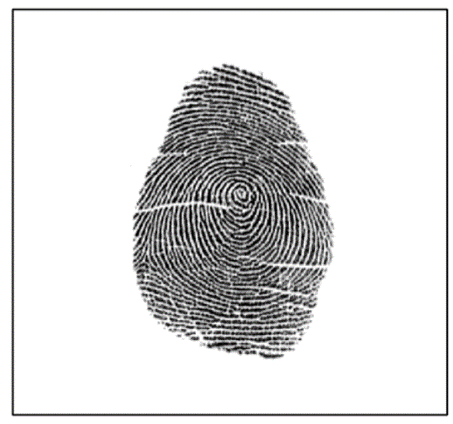
\includegraphics[height=0.45\textwidth]{img/chapter_br/fingerprint_img.png}}
\caption{指纹采集设备和图像\cite{maltoni2009handbook}}
\label{fig:fingerprint}
\end{figure}

掌纹识别是近些年提出的一种相对较新的生物特征识别技术。掌纹一般指手指末端到手腕之间这一区域的手掌表面的各种纹理特征,如图\ref{fig:palmprint_img}所示。与指纹识别类似,每个人的掌纹纹理都不一样,掌纹中具有的很多特征可以进行测量并提取特征值,进而进行身份认证。指纹识别和掌纹识别都是非侵犯性的识别方法,实际应用中用户接受度较高。

\begin{figure}[ht]
\centering  %图片全局居中
\subfigure[掌纹采集设备]{
\label{fig:palmprint_equip}
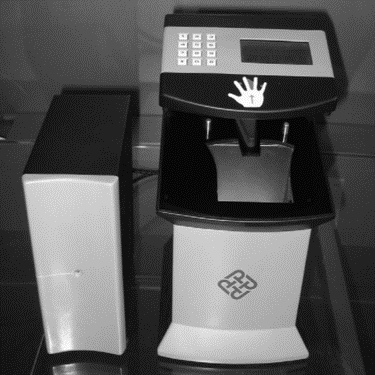
\includegraphics[height=0.45\textwidth]{img/chapter_br/palmprint_equip.png}}
\subfigure[掌纹图像]{
\label{fig:palmprint_img}
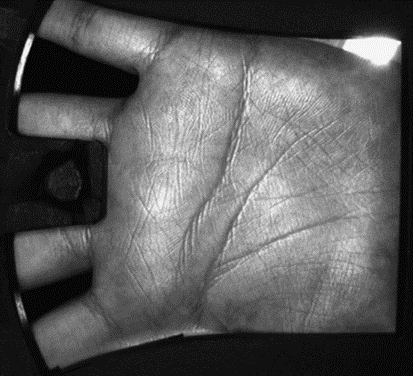
\includegraphics[height=0.45\textwidth]{img/chapter_br/palmprint_img.png}}
\caption{掌纹采集设备和图像\cite{kong2009survey}}
\label{fig:palmprint}
\end{figure}

\section{静脉识别}
静脉识别利用的是静脉中的血红蛋白相对于肌肉、骨骼等其他生理组织对近红外光的吸收率更高,当有近红外光照射在手指或者手掌上时,通过红外摄像头获取手指或手掌的图像,静脉血管会呈现深色,肌肉组织则为浅色,呈现出黑白对比分明的图像特点,如图\ref{fig:finger_vein}所示,静脉血管结构可以清晰的得到呈现。静脉识别技术通过算法对图像进行分析,提取特征值进行身份认证。静脉采集设备按照近红外光源和图像传感器的相对位置不同,主要分为透射式和反射式两种,如图\ref{fig:finger_vein_equip}所示。

\begin{figure}[ht]
\centering  %图片全局居中
\subfigure[指静脉反射式成像]{
\label{fig:finger_vein_1}
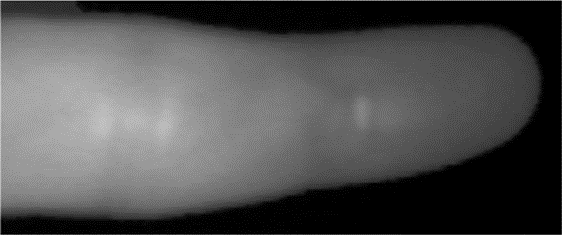
\includegraphics[width=0.65\textwidth]{img/chapter_br/finger_vein.png}}
\subfigure[指静脉透射式成像]{
\label{fig:finger_vein_2}
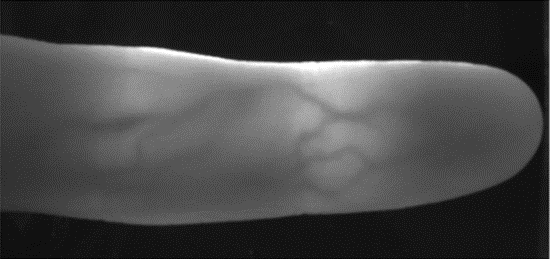
\includegraphics[width=0.65\textwidth]{img/chapter_br/finger_vein_2.png}}
\caption{指静脉图像\cite{hashimoto2006finger}}
\label{fig:finger_vein}
\end{figure}

\begin{figure}[ht]
\centering
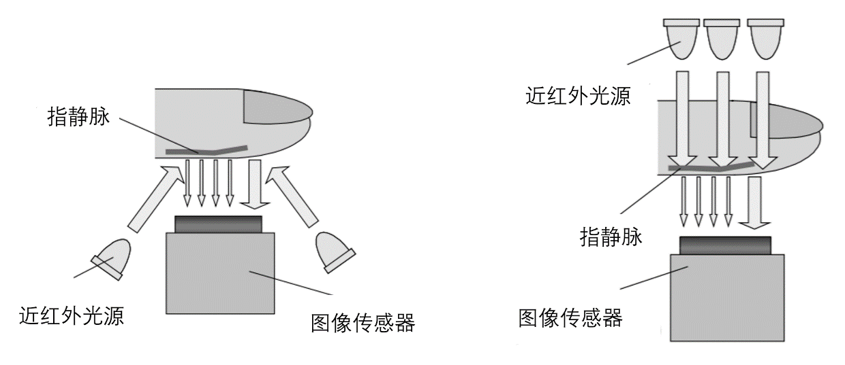
\includegraphics[scale=0.6]{img/chapter_br/finger_vein_equip.png}
\caption{两种指静脉图像采集方式示意图\cite{hashimoto2006finger}}
\label{fig:finger_vein_equip}
\end{figure}

由于静脉属于人体内部特征,相比人脸和指纹来说极难复制和盗取,且只有在活体上才能采集到,因此这项技术的安全性更好,更难以被盗取和假冒。静脉识别过程中一般受外界环境因素(例如温度、湿度等)以及个体皮肤表面状态(如粗糙程度、是否磨损等)影响较小,可靠性较高。同时在使用过程中,用户手无需与设备进行接触,这种非接触式的使用更加卫生、易于用户接受。目前静脉识别技术发展时间较短,识别准确率有望进一步得到提升。由于在活体鉴定方面的优势,与指纹融合可以较好地预防假指纹攻击,并提高识别准确率。
静脉识别在金融行业的应用也已开始了探索。2016年1月,工农中建四大银行委托广电运通起草指静脉在金融行业的应用标准。2016年11月,广东省社保基金管理局也已经制定指静脉在社保行业的应用标准,计划全省开始推广指静脉养老金发放的认证工作。

\section{虹膜识别}

虹膜是位于人眼表面黑色瞳孔和白色巩膜之间的圆环状区域,在近红外光下能够呈现出丰富的纹理,如图\ref{fig:iris_img}所示。而且虹膜在胎儿发育阶段形成后的整个生命历程中是保持不变的。这些特征决定的虹膜特征以及用于身份识别的唯一性。虹膜识别属于非接触式识别,通过专门的虹膜图像采集装置采集清晰的虹膜图像提取特征进行身份认证,识别过程高效且准确率高。虹膜识别技术被认为是生物特征识别技术中准确率最高的技术之一,在金融领域一般应用于金库管理、押运管理的较多,通过虹膜识别确认出入和押运人员身份,确保财产安全;同时,也有部分银行在尝试将虹膜识别和指静脉识别集成于自助终端中,实现更高安全级别的身份认证,以帮助用户完成自助贷款、自助理财等业务的办理。在其他行业,虹膜识别技术因眼镜、光线干扰和特征部位与采集方式等因素,目前主要用于煤矿工人等其他种类生物特征难以采集和识别的人群。

\begin{figure}[ht]
\centering
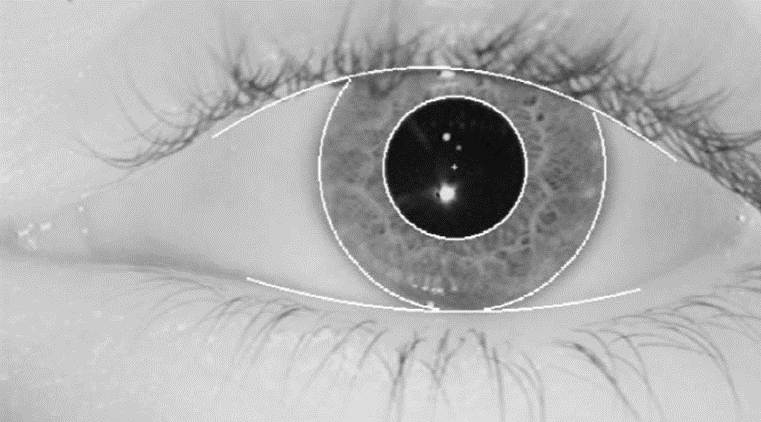
\includegraphics[scale=0.6]{img/chapter_br/iris_img.png}
\caption{虹膜图像\cite{daugman2009iris}}
\label{fig:iris_img}
\end{figure}

以上是目前较为常见的几种生物特征识别技术。随着智能终端设备以及生物特征传感器的快速普及和优化,生物特征识别技术已经进入大规模应用阶段。单一的人脸识别或指纹识别已经难以满足金融机构的多样化需求,多模态生物识别是金融科技不可更改的趋势。